\documentclass[tikz,border=10pt]{standalone}
\usepackage{tkz-euclide} % 增强几何绘图功能

\begin{document}
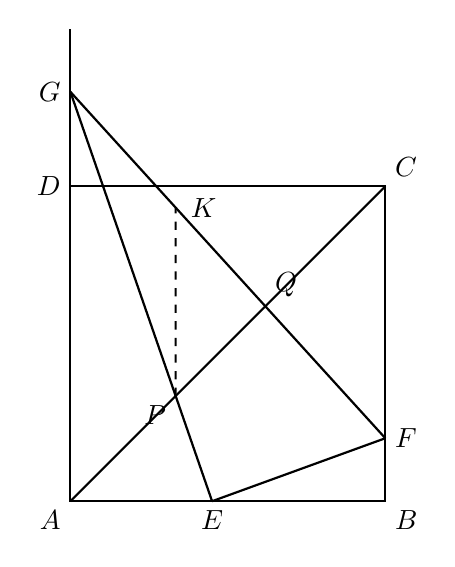
\begin{tikzpicture}[scale=4, >=stealth]
    % 1. 定义正方形的四个顶点
    \coordinate (A) at (0,0);
    \coordinate (B) at (1,0);
    \coordinate (C) at (1,1);
    \coordinate (D) at (0,1);

    % 2. 定义外部点与辅助点 (基于图像比例估算：E约在AB的1/2处，F约在BC的1/4处，G在AD延长线上)
    \coordinate (E) at (0.45, 0);
    \coordinate (F) at (1, 0.2);
    \coordinate (G) at (0, 1.3);

    % 3. 绘制正方形边界
    \draw[thick] (A) -- (B) -- (C) -- (D) -- cycle;

    % 4. 绘制AD的延长线
    \draw[thick] (D) -- (0, 1.5);

    % 5. 绘制内部连线
    \draw[thick] (A) -- (C);          % 对角线 AC
    \draw[thick] (G) -- (E);          % 连线 GE
    \draw[thick] (E) -- (F);          % 连线 EF
    \draw[thick] (G) -- (F);          % 连线 GF

    % 6. 计算并标记交点 P (AC 与 GE 的交点)
    \coordinate (P) at (intersection of A--C and G--E);
    % 计算并标记交点 Q (AC 与 GF 的交点)
    \coordinate (Q) at (intersection of A--C and G--F);

    % 7. 绘制虚线辅助线 PK (K 在 GF 上，PK 垂直于 x 轴)
    % 先找到 K 点：过 P 作垂直线与 GF 相交
    \coordinate (K) at (P |- 0, 0.85); % 初始估计 K 的位置
    % 修正 K 点：使其严格落在 GF 连线上
    \coordinate (K) at (intersection of P--[shift={(0,1)}]P and G--F);
    \draw[thick, dashed] (P) -- (K);

    % 8. 标注各点文字
    \node[below left] at (A) {$A$};
    \node[below right] at (B) {$B$};
    \node[above right] at (C) {$C$};
    \node[left] at (D) {$D$};
    \node[below] at (E) {$E$};
    \node[right] at (F) {$F$};
    \node[left] at (G) {$G$};
    \node[below left] at (P) {$P$};
    \node[above right] at (Q) {$Q$};
    \node[right, xshift=2pt] at (K) {$K$};

    % 9. 可选：绘制直角标记（如 A 点）
    %\draw (0.05,0) -- (0.05,0.05) -- (0,0.05);

\end{tikzpicture}
\end{document}